\documentclass[tikz]{standalone} 

\usepackage{newtxtext,newtxmath}

%!TEX root = main.tex

% mytikzset
\usepackage{tikz}
\usetikzlibrary{positioning,arrows,shapes,patterns}
\usetikzlibrary{decorations.pathmorphing}
\usetikzlibrary{decorations.markings}
\usetikzlibrary{decorations.pathreplacing}
\usetikzlibrary{calc}
\usetikzlibrary{patterns}
\usetikzlibrary{decorations.markings}
\usetikzlibrary{petri}

\tikzset{
  vector/.style={thick,double,draw=black, postaction={decorate},
    decoration={markings,mark=at position .6 with {\arrow[black,scale=0.4]{triangle 45}}}},
  axial/.style={thick,double,densely dashed,draw=black, postaction={decorate},
    decoration={markings,mark=at position .6 with {\arrow[black,scale=0.4]{triangle 45}}}},
  gluon/.style={decorate, draw=black,
    decoration={coil,aspect=0.3,segment length=5pt,amplitude=3pt}},
  pseudo/.style={thick, dashed, draw=black, postaction={decorate},
    decoration={markings,mark=at position .6 with {\arrow[red,scale=0.5]{triangle 45}}}},
  scalar/.style={thick,draw=black, postaction={decorate},
    decoration={markings,mark=at position .6 with {\arrow[black,scale=0.5]{triangle 45}}}},
  cut/.style={draw=black, decorate, decoration={snake, segment length=1mm, amplitude=0.2mm}}
}

\definecolor{myGreen}{RGB}{0,127,0}

\begin{document}
\nopagecolor
  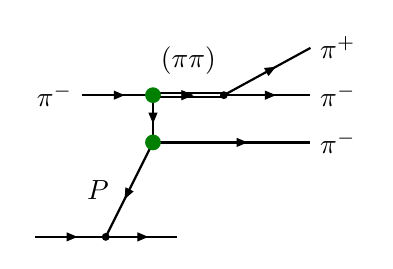
\begin{tikzpicture}[node distance=0.6cm and 0.9cm, baseline=1cm]
    \coordinate[] (a1);
    \coordinate[	right=of a1] (a2);
    \coordinate[right=of a2] (a3);
    \coordinate[above =of a2, xshift=3mm] (z1);
    \coordinate[above =of z1, xshift=3mm] (z2);
    \coordinate[right=of z2] (z3);
    \coordinate[above=of z2] (b12);
    \coordinate[left=of b12, label=left:{$\pi^{-}$}] (b1);
    \coordinate[right=of b12] (b2);
    \coordinate[      right=of b2,xshift=2mm,label=right:$\pi^-$] (b3);
    \coordinate[above right=of b2,xshift=2mm,label=right:$\pi^+$] (b4);
    \coordinate[below right=of b2,xshift=2mm,label=right:$\pi^-$] (b5);
    
    \draw[scalar]  (a1) -- (a2);
    \draw[scalar]  (a2) -- (a3);
    \draw[scalar]  (b12) -- (z2);
    \draw[scalar]  (z2) -- node[label=left:{$\mathbb{P}$}] {} (a2);
    \draw[scalar]  (b1) -- (b12);
    \draw[vector]  (b12) -- node[label=above:{$(\pi\pi)$}] {} (b2);
    \draw[scalar]  (b2) -- (b3);
    \draw[scalar]  (b2) -- (b4);
    \draw[scalar]  (z2) -- (b5);
    \fill[myGreen] (b12) circle [radius=0.1];
    \fill[myGreen] (z2) circle [radius=0.1];
    \fill[black] (b2) circle [radius=0.05];
    \fill[black] (a2) circle [radius=0.05];
  \end{tikzpicture}
\end{document}
